\documentclass[../uilmath.tex]{subfiles}
\graphicspath{{\subfix{../figures/}}}
\begin{document}
\chapter{Calculus}
\section*{Problems}
\begin{enumerate}[label=\bfseries\arabic*.]
    \item %% Problem 1
    Find the area of the shaded region (nearest square unit)
    \begin{center}
        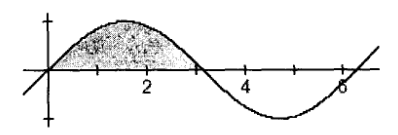
\includegraphics[width=0.3\textwidth]{2006SAC20.PNG}
    \end{center}

    \item %% Problem 2
    Which of the following sequences is divergent?

    $\textbf{(A) } \left\{\frac{2n+1}{3n-2}\right\}\qquad \textbf{(B) }\left\{\frac{-1^n}{n^2+n}\right\}\qquad \textbf{(C) }\left\{\frac{(-1)^n(n+1)}{n+2}\right\}\qquad \textbf{(D) }\left\{\frac{4n^2-n^3}{10+2n^3}\right\}\qquad \textbf{(E) }\left\{\frac{6n^2+3n-1}{n^2+8n+16}\right\}$

    \item %% Problem 3
    If $f'(x)=6x^2-4x+1$ and $f(1)=0$, find $f(-1)$.

    \item %% Problem 4
    $f(x)=2x^3-6x+1$ has an inflection point at:
    
    \item %% Problem 5
    Find the area (in square units) of the region bounded by $x=\frac{y^2+2}{2}$ and $x=y+5$.

    \item %% Problem 6
    The graph of $f'(x)$ is shown below. If $f(1)=2\frac{1}{3}$, then $f(2)=\blank$.
    \begin{center}
        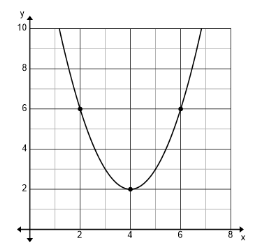
\includegraphics[width=0.3\textwidth]{2021SAC9.PNG}
    \end{center}
    
    \item %% Problem 7
    The point of inflection for the graph of $f(x)$ has coordinates $(a,b)$. $a+b=\blank$. (nearest tenth)

    \begin{center}
        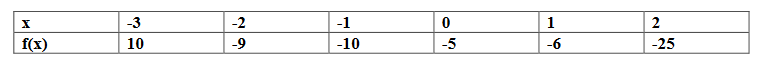
\includegraphics[width=0.8\textwidth]{2021SAC26.PNG}
    \end{center}



    The following graph is used for problems 8 and 9.
    \begin{center}
        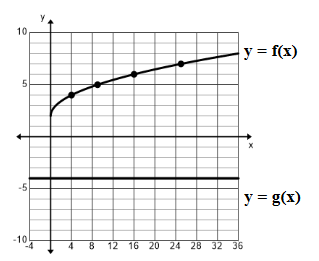
\includegraphics[width=0.3\textwidth]{2021SAC42.PNG}
    \end{center}
    \item %% Problem 8
    Find the area between the curves $y=f(x)$ and $y=g(x)$ shown on the right over the interval $[4,24]$. (nearest whole number)

    \item %% Problem 9
    Find the volume of the solid generated by revolving the region bounded by $y=f(x)$, the $x$-axis, the line $x=4$ and 
    the line $x=24$ about the line $y=g(x)$. (nearest whole number)

    \item %% Problem 10
    Find the area of one petal of the rose curve $r=6\cos(2\theta)$. (nearest tenth)

    \item %% Problem 11
    Find the interval of convergence for the power series $\sum_{n=1}^\infty \frac{(-1)^{n+1}x^n}{4^n}$.

    \item %% Problem 12
    Find the value of $c$ in the open interval $(-8,2)$ that satisfies the mean value theorem for the function 
    $f(x)=\sqrt{6-x}$. (nearest hundredth)

    \item %% Problem 13
    If you were going to evlauate $\int \frac{\cos x}{\sin^3 x}\mathrm{d}x$ using $u$-substitution, the best choice for $u$ is \blank.

    \item %% Problem 14
    If $f(x)=x^2-8x+9$, then $\frac{f(x+h)-f(x)}{h}=\blank$.

    \item %% Problem 15
    Find the area bounded by thw two curves shown below. (nearest tenth)
    \begin{center}
        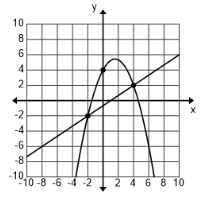
\includegraphics[width=0.3\textwidth]{2022SAC40.PNG}
    \end{center}

    \item %% Problem 16
    Consider the function $f(x)=\frac{1}{2}\cos(2x)+\frac{3}{2}\sin(x)$. Find the slope of the line tangent to 
    the graph of $y=f(x)$ when $x=\pi$. (nearest tenth)

    \item %% Problem 17
    A balloon is rising straight up from a point on the ground 150 feet from a curious mouse. If the balloon is rising at a 
    rate 8 ft/s, what is the rate of change of the angle of elevation of the balloon from the mouse when the balloon is 200 ft above the groud. (nearest hundredth)

    \item %% Problem 18
    A rectangular solid with a square base has a total surface area of 330 in$^2$. Find the maximum volume possible for such a solid. (nearest tenth)


    Use the following graph for questions 19 and 20.
    \begin{center}
        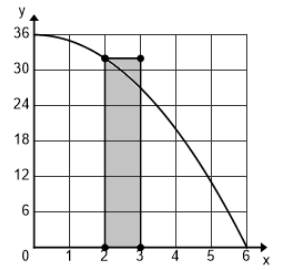
\includegraphics[width=0.3\textwidth]{2022SAC45.PNG}
    \end{center}
    \item %% Problem 19
    Find an approximation of the area bounded by the graph of $f(x)=36-x^2$ and the $x$-axis between $x=1$ and $x=5$. 
    Use four rectangles of equal width and find the height of each rectangle using the left endpoint of the interval. One of the rectangles is shown above.

    \item %% Problem 20
    Find the exact area of the region bounded by the graph of $f(x)=36-x^2$ and the $x$-axis between $x=1$ and $x=5$. (nearest tenth)

    \item %% Problem 21
    Find the derivative of $F(x)$ if $F(x)=\int_0^{4x}\sin(t)\mathrm{d}t$.

    \item %% Problem 22
    When evaluating $\int x^2\cos(x)\mathrm{d}x$ using a $u$-substitution, the best choice for $u$ is $\blank$.

    \item %% Problem 23
    Let $f(x)=\sin(x)$ and let $P_5(x)$ be the fifth Maclaurin polynomial for $f(x)=\sin(x)$. Find the value of 
    $\left|P_5\left(\frac{\pi}{6}\right)-f\left(\frac{\pi}{6}\right)\right|$. (nearest ten-millionth)

    \item %% Problem 24
    Find the length of the arc from $\theta=\frac{\pi}{6}$ to $\theta=\frac{\pi}{3}$ for the polar curve $r=4-4\cos(\theta)$. (nearest tenth)

    \item %% Problem 25
    The point $A(6,b)$ lies on the graph of the parametric equations $x(t)=\sqrt{2t}$ and $y(t)=\frac{10}{t+2}$, $0\leq t\leq 60$.
    $b=\blank$.


    The following graph is used for problems 26 and 27.
    \begin{center}
        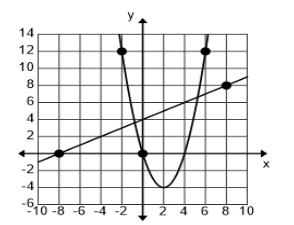
\includegraphics[width=0.3\textwidth]{2023SAC40.PNG}
    \end{center}
    \item %% Problem 26
    The points of intersection of the curves shown on the right are $P$ and $Q$. $PQ=\blank$. (nearest tenth)

    \item %% Problem 27
    Find the area bounded by the two curves shown on the right. (nearest tenth)

    \item %% Problem 28
    The \blank Theorem states that ``If $f$ is a continuous, real valued function defined on an interval $[a,b]$, 
    with $f(a)\neq f(b)$, and $k$ is a real number between $f(a)$ and $f(b)$, then there exists some $c\in (a,b)$ such that $f(c)=k$.''

    \item %% Problem 29
    Emmitt won the lottery and decided to purchase some land near Lubbock and raise emus. He wanted to build a pen in the 
    shape of a rectangle to keep his emus. He has 480 feet of fencing to use for three sides of the pen. He will use one side of 
    his large barn as the fourth side. What is the maximum area of the pen? (nearest square foot)

    \item %% Problem 30
    An 18-ft-long ladder rests against the wall of a building. The foot of the ladder begins to slide away from the building at a constant rate of 6 in/s. How fast is the 
    top of the ladder sliding down the wall at the instant the ladder makes an angle of $30\degree$ with the wall? (nearest hundredth)

    \item %% Problem 31
    Find the area of the region in the first quadrant bounded by the graphs of $y_1=3+\cos(x)$ and $y_2=2-\cos(x)$ and the $y$-axis. (nearest tenth)

    \item %% Problem 32
    Find the slope of the line tangent to the curve $2y^2-6xy+3x^3-4y=8$ when $x=1$ and $y>0$. (nearest hundredth)

    \item %% Problem 33
    To evaluate $\int \sin^5(x)\cos(x)\mathrm{d}x$ using a $u$-substitution, the best choice for $u$ is \blank.

    \item %% Problem 34
    To evaluate $\int x^2\sin(x)\mathrm{d}x$ using integration by parts, the best choice for $u$ is \blank.

    \item %% Problem 35
    Experts from Texas Tech believe that Newberry State Park in Seminole is capable of supporting no more than 250 prairie dogs.
    On April 1, 2012, Anthony introduced the first pair of prairie dogs. On April 1, 2020 the population had reached 60 prairie dogs.
    Professor Cravens commissioned Carter to develop a logistic model of the prairie dog population. The logistic model predicts that there should be 
    about \blank prairie dogs in 2030.


    For problems 36 and 37, consider the curve given by $x(t)=\sin(t)$ and $y(t)=t+\cos(t)$, $\frac{\pi}{2}\leq t\leq \frac{5\pi}{2}$. (rad)
    \item %% Problem 36
    Find the length of the curve. (nearest hundredth)

    \item %% Problem 37
    The tangent line when $t=\pi$ intersects the tangent line when $t=2\pi$ at the point $P(a,b)$. $a+b=\blank$. (nearest hundredth)


    For problems 38-41, consider the following graph.
    \begin{center}
        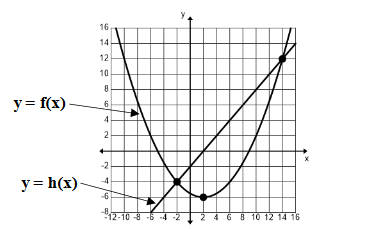
\includegraphics[width=0.6\textwidth]{2024SAC39.PNG}
    \end{center}
    \item %% Problem 38
    The graphs of $y=f(x)$ and $y=h(x)$ intersect at the points $P$ and $Q$. $PQ=\blank$. (nearest tenth)

    \item %% Problem 39
    The point $F(2,b)$ is the focal point of the parabola. $b=\blank$.

    \item %% Problem 40
    The area bounded by the graphs of $y=f(x)$ and $y=h(x)$ is $\blank$. (nearest tenth)

    \item %% Problem 41
    If the area bounded by the graphs of $y=f(x)$ and $y=h(x)$ is revolved around the line $x=-6$, then the volume 
    of the solid generated is \blank. (nearest whole number)

    \item %% Problem 42
    Consider the graph of $h(x)=2\ln(x)-\frac{1}{e^x}$. The slope of the line tangent 
    to the graph of $h(x)$ at $x=9$ is \blank. (nearest thousandth)

    \item %% Problem 43
    Consider the graph of $2xy^2-3y+4x^2=13$. The $y$-intercept of the line tangent to the curve at the point where $y=3$ and $x>0$ is \blank. (nearest tenth)

    \item %% Problem 44
    Farmer Fred wants to make a rectangular holding area for his dairy cattle using 640 feet of fence. He plans to use the 
    back side of his barn as one of the sides. The maximum possible value of the holding area is \blank square feet.

    \item %% Problem 45
    A 25-ft-long ladder rests against the wall of a building. The foot of the ladder begins to slide away from the building at a constant rate of 2 ft/s. How fast 
    is the top of the ladder sliding down the wall at the instant the foot of the ladder is 7 feet from the wall? (nearest whole number)

    \item %% Problem 46
    The position of a particle is given by the parametric equations $x(t)= e^{.4t}$ and $y(t)=\ln(t^2+2)$ for $0\leq t\leq 12$. Find the 
    total distance traveled by the partial from $t=2$ to $t=10$. (nearest tenth)


    Use the following graph for problems 47 and 48.
    \begin{center}
        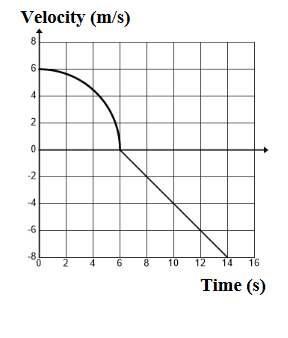
\includegraphics[width=0.3\textwidth]{2024SAC48.PNG}
    \end{center}
    The graph consists of a quarter circle and a line segment. The graph represents the velocity of an object during a 14-second time interval.
    \item %% Problem 47
    Find the object's average velocity during the 14-second time interval $[0,14]$. (Nearest hundredth)

    \item %% Problem 48
    Find the objects acceleration at $t=10$ s.


    \begin{center}
        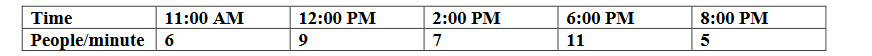
\includegraphics[width=0.8\textwidth]{2024SAC50.PNG}
    \end{center}
    \item %% Problem 49
    Suppose that Larry's Cafeteria in Millersview opens their doors at 11:00 AM and closes their doors at 8:00 PM.
    The table above shows the rate at which people entered the cafeteria, in people per minute, at various times on Saturday.
    Use a trapezoidal approximation with four subintervals to estimate the total number of people who dined at Larry's on Saturday.

    \item %% Problem 50
    The rate of change of a population of horned lizards at any time $t$, $t\geq 0$, is changing at a rate proportional to 
    its population at time $t$. The population on March 1, 2000 was 180. On March, 1, 2004 the population was 210. What should the population be on March 1, 2033?

    \item %% Problem 51
    Consider the curve given by $f(x)=x^3+6x^2-4x+2$. The local maximum of $f(x)$ is \blank. (nearest tenth)

    \item %% Problem 52
    $\int 2^{-x}\mathrm{d}x=\blank + C$, where $C$ is an arbitrary constant.

    \item %% Problem 53
    $\int \frac{13}{144+25\cos^2 x}\mathrm{d}x=\frac{1}{b}\tan^{-1}(\frac{b}{c}\tan x)+C$ where $C$ is an arbitrary constant,
    $c>b>a>0$ and $a,b,c$ form a primitive Pythagorean triple. Find $a$.

    \item %% Problem 54
    The function $f(x)=x^3-3x^2+3$ has an inflection point at:

    \item %% Problem 55
    The area (in square units) of the region bounded by $y=1-x^2$ and the $x$-axis is:

    \item %% Problem 56
    Let $f$ be a function such that it is continuous on $[a,b]$ and it is differentiable on $(a,b)$.
    Then there exists at least one number $c$ in $(a,b)$ such that $f'(c)=\frac{f(b)-f(a)}{b-a}$. This theorem is known as:

    \item %% Problem 57
    Let $f(x)=
    \begin{cases}
        x & \text{ if } x\leq 0 \\
        x^2 & \text{ if } 0<x 
    \end{cases}$
    Which of the following statements is a false statement.

        $\textbf{(A) }$ $f$ is continuous at 0 \qquad \textbf{(B) } the right hand derivative at 0 is 0 \\
        $\textbf{(C) }$ the left hand derivative at 0 is 1 \qquad \textbf{(D) } $f$ is not differentiable at 0 \textbf{(E) } $f(-1)=f(1)$

    \item %% Problem 58
    Find the area, in square units, of the figure bounded by $y=x^2-x-2$ and below the $x$-axis.

    \item %% Problem 59
    Let $f(x)=\frac{x-2}{3x+5}$. Find $f'(-1)$.

    \item %% Problem 60
    Find the digit in the ten-thousandths place of the series $1+x+\frac{x^2}{2!}+\frac{x^3}{3!}+\frac{x^4}{4!}+\dots$, when $x=\pi$.

    \item %% Problem 61
    A function $y=f(x)$ is continuous on $[a,b]$, if $f(a)<y_0<f(b)$ then $y_0=f(c)$ for some $c$ in $[a,b]$. This theorem is the: 

    \item %% Problem 62
    Let $f(x)=ax^5-bx^4-bx^3+ax^2+ax-b$. Find $f''(1)$.

    \item %% Problem 63
    If $a_1=-4, a_3=-9$, and $a_4=13.5$ are terms of a geometric sequence, then $a_2=\blank$.

    \item %% Problem 64
    How many points of intersection occur when $r=2\cos\theta+1$ and $\theta=\pi$ are graphed on a polar coordinate system?

    \item %% Problem 65
    \[\sum^2_{k=0}(kx+(k+1)y)=\]

    \item %% Problem 66
    Find the area of the shaded region in square units.
    \begin{center}
        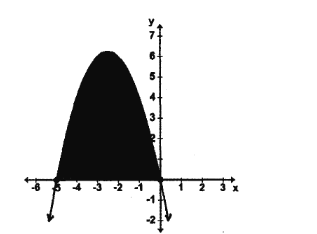
\includegraphics[width=0.4\textwidth]{2009A40.PNG}
    \end{center}

    \item %% Problem 67
    If $f(x)=\frac{2x+3}{4x-5}$, then $f'(1)=\blank$

    \item %% Problem 68
    The slope of the line tangent to the curve $y=2x^3-3x^2-5$ at $x=2$ is 12. The point of intersection of the tangent line and curve is:

    \item %% Problem 69
    Evaluate $\int^n_{-n}(x^3-3x^2-5)\mathrm{d}x$

    \item %% Problem 70
    Find $f(2)$ when $f(x)=1-\frac{x^2}{2}+\frac{x^4}{24}-\frac{x^6}{720}+\dots$. (nearest thousandth)

    \item %% Problem 71
    Let $f$ be a function such that it is differentiable on $(a,b)$ and continuous on $[a,b]$, and $f(a)=f(b)=0$. Then there is a number 
    $c$ in $(a,b)$ for which $f'(c)=0$. This theorem is known as: 

    \item %% Problem 72
    The function $f(x)=\frac{2}{x-1}+18x$ is increasing at which of the following values of $x$?

    \item %% Problem 73
    Find the area (in square units) of the region bounded by $y=-x^2$ and $y=-4$.

    \item %% Problem 74
    Let $f(x)=\frac{4x+5}{3x}$. Find $f'(2)$.

    \item %% Problem 75
    Find an equation of the tangent line to the curve $y=\sqrt{9-4x}$ at the point $(-4,5)$.

    \item %% Problem 76
    The point of inflection on the graph of $f(x)=2x^3-6x^2+6x-6$ is $(a,b)$. Find $b$.

    \item %% Problem 77
    Find an equation of the line tangent to the curve $y=x^3-2x^2$ at the point $(1,-1)$.

    \item %% Problem 78
    The area (in square units) of the region bounded by $y=-x^2-4x$ and $y=0$ is: 

    \item %% Problem 79
    $\int (-x\sin x)\dd x=\blank +C$, where $C$ is some arbitrary constant.

    \item %% Problem 80
    If $f''(x)=6$ and $f'(-1)=-8$ and $f(1)=2$, then $f(-2)=\blank$ .

    \item %% Problem 81
    Find the instantaneous rate of change of the reciprocal of a number with respect to the number when the number is 4.

    \item %% Problem 82
    Let $f(x)=\frac{1}{x-1}$. Find the average rate of change of $f(x)$ over the interval $[2,5]$.

    \item %% Problem 83
    Find the first term of the geometric sequence: $a,b,44,c,19\frac{5}{9},\dots$

    \item %% Problem 84
    If $f'(x)=15x^2-6x+2$ and $f(-1)=-9$, find $f(1)$.

    \item %% Problem 85
    $\int \sin(2x)\cos(2x)\dd x=\blank +C$, where $C$ is an arbitrary constant.

    \item %% Problem 86
    Elmoor Fudd is building a rectangular shaped pen for his porkie pigs. It will have 4 parallel fences dividing the pen into 5 sections as shown. If he has 600 feet of fencing, what is the maximum area of his pig pen?
    \begin{center}
        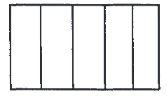
\includegraphics[width=0.4\textwidth]{2010B54.PNG}
    \end{center}

    \item %% Problem 87
    Find the area of the region bounded by the graphs of $x=4-y^2$ and $x=4-4y$.

    \item %% Problem 88
    If $f'(x)=3x^2-5$ and $f(-1)=4$, find $f(1)$.

    \item %% Problem 89
    Let $\frac{1}{x}+\frac{1}{y}=1$. Find $D_x y$.

    \item %% Problem 90
    What is the instantaneous rate of change at $x=2$ of the function $f$ given by $f(x)=\frac{x^2-2}{x-1}$

    \item %% Problem 91
    Let $f(x)=\begin{cases}
        3 + x & \text{ if }x\leq 1 \\
        3-x & \text{ if }1 < x 
    \end{cases}$. Which of the following is/are true? 
    \[ 1. \lim_{x\to 1^+} f(x) \text{ exists } \qquad 2. \lim_{x\to 1^-} f(x) \text{ exists} \qquad 3. f(x) \text{ is continuous}\]

    \item %% Problem 92
    The function $f(x)=\begin{cases}
        nx^3-x \text{ if } x\leq 1 \\
        mx^2+5 \text{ if } 1<x 
    \end{cases}$ is differentiable everywhere. Find $n$.

    \item %% 93
    Let $f(x)=\frac{5x-2}{4+3x}$. Find $f'(-2)$.

    \item % 94
    Find the value of $\int_{-1}^4 f(x)\dd x$ for the piecewise-linear function, $f$, $-1\leq x\leq 4$, shown below?
    \begin{center}
        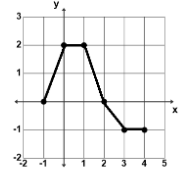
\includegraphics[width=0.4\textwidth]{2018B24.PNG}
    \end{center}

    \item % 95
    Mei Chado is 5' 4'' tall. She is walking at a rate of 3 ft/sec toward a street light that is 16 feet tall. At what rate is the tip of her shadow moving? (nearest tenth)

    \item % 96
    Let $f(x)=4x^2-4x+1$. The tangent to $f(x)$ at $(x,y)$ is parallel to $y=4x-2$. Find $x+y$.

    \item % 97
    Let $f(x) = \begin{cases}
        -x+5 \qquad x<-2 \\ 
        x^2+1 \qquad -2\leq x \text{ and } x\leq 1 \\ 
        2x^3-1 \qquad 1\leq x
    \end{cases}$. Which of the following is/are true?

    \begin{enumerate}
        \item $f$ is continuous at $-2$
        \item $f$ is differentiable at $x=1$
        \item $f$ has a local minimum at $x=0$
    \end{enumerate}

    \item % 98
    A cable is connected from the shorter tower to the taller tower. What is the minimum length of the cable? (nearest inch)
    \begin{center}
        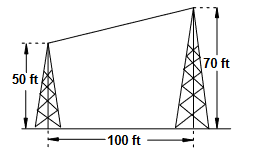
\includegraphics[width=0.3\textwidth]{2019A25.PNG}
    \end{center}

    \item % 99
    Find the area bounded by $f(x)=x^3, f(y)=-2$, and $f(y)=1$. (square units)

    \item % 100
    What is the slope of the secant line to the graph of $f(x)=2x^2+3x-4$ passing through the points $(1,m)$ and $(-3,n)$?

    \item % 101
    Rusty Pipes has a leaky pipe dripping water onto the floor forming a circular pool. The radius of the pool increases at a rate of 4 cm/min.
    How fast is the area of the pool increasing when the radius is 5 cm? (nearest cm$^2$/min)

    \item % 102
    Let $f''(x)=12x-6, f'(0)=4$, and $f(0)=-5$. Find $f(1)$.

    \item % 103
    Let $f(x)=|x-5|$. How many of the following statements are always true?

    \[ \textbf{a. } \lim_{x\to 5^+} f(x)\text{ exists} \qquad \textbf{b. } \lim_{x\to5^-} f(x)\text{ exists}\qquad \textbf{c. } f(x) \text{ is continuous} \qquad \textbf{d. } f(x) \text{ is differentiable}\] 

    \item % 104
    The partial fraction decomposition of $\frac{x+8}{x^2+x-6}$ is $\frac{A}{x-2}+\frac{B}{x+3}$. $A+B=\blank$.


    The following graph is used for problems 105, 106, 107, and 108. 
    \begin{center}
        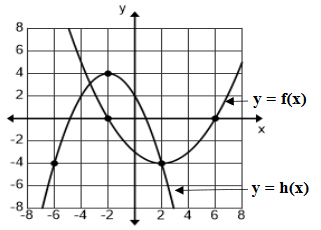
\includegraphics[width=0.3\textwidth]{2023D39.PNG}
    \end{center}
    \item % 105
    The directrix of the graph of $y=h(x)$ is the line $y=c$. The value of $c$ is \blank .

    \item % 106
    If the parabolas intersect at points $A$ and $B$, then $AB=\blank$. (nearest tenth)

    \item % 107
    The area of the region bounded by the graphs of the parabolas is \blank . (nearest tenth)

    \item % 108
    Find the arc length of the graph of $y=f(x)$ on the interval $[0,8]$. (nearest tenth)

    \item % 109
    A rectangle is to be inscribed between the graph of $y=16-x^2$ and the $x$-axis with its base on the $x$-axis. What is the maximum area of such a rectangle? (nearest tenth)

    \item % 110
    Find the sum of the series. $2-\frac{4}{3}+\frac{4}{15}-\frac{8}{315}+\dots$

    \item % 111
    Find the area in the second quadrant bounded by the $x$-axis, the $y$-axis, and the graph of $r(\theta)=2\theta+3\sin(theta), 0\leq\theta\leq 2\pi$. (nearest tenth)


    The following graph is used for problems 112 and 113.
    \begin{center}
        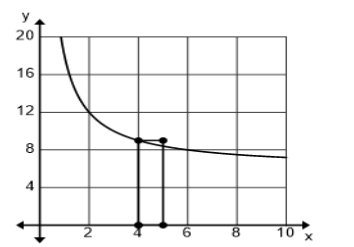
\includegraphics[width=0.3\textwidth]{2023D46.PNG}
    \end{center}
    \item % 112
    Consider the graph of $y_1 = \frac{12}{x}+6$. Use the Left Rectangle Approximation Method with six rectangles of equal width to approximate the area bounded by the curves 
    $y_1=\frac{12}{x}+6, y_2=0, x_1=2$, and $x_2=8$. One of the rectangles is shown above. (nearest hundredth)

    \item % 113
    Find the volume of the solid generated when the region bounded by the curves $y_1=\frac{12}{x}+6, y_2=0, x_1=2,x_2=8$ is revolved around the line $x=12$. (nearest whole number)

    \item % 114
    The Panhandle Coffee shop keeps their dining area at a constant $72\degree$. They serve their famous coffee at exactly $175\degree$ and the 
    temperature of the coffee changes at the rate $r(t)=-5.89e^{-.0766t}$ degrees per minute. Darius received a phone call at the moment his coffee was 
    served and his coffee cooled for exactly five minutes before he was able to take his first sip. What was the temperature of the coffee when he took his first sip? (nearest whole number)

    \item % 115
    (rad) The derivative of the function $f$ is given by $f'(x)=2x^3-6\sin(x^2)+2$. On the interval $(-2,2)$, at which of the following values does $f$ have a relative minimum? (nearest thousandth)

    $\textbf{I.} -0.535 \qquad \textbf{II. } 0.669 \qquad \textbf{III. } 1.260$


    For problems 116 and 117 use the following information:

    (rad) The position of an object moving in the $xy$-plane is given by $(x(t),y(t)), 0\leq t\leq \frac{5\pi}{12}$, with $\frac{\dd x}{\dd t} = 4t\sin(t)$ cm/s and 
    $\frac{\dd y}{\dd t} = 4t\cos(t)$ cm/s. At $t=0$, the position of the object is $(4,8)$.
    \item % 116
    Find the speed of the object at $t=\frac{\pi}{6}$. (nearest hundredth)

    \item % 117
    The position of the object at $t=\frac{\pi}{3}$ is $(a,b)$. $b=\blank$. (nearest hundredth)

    \item % 118
    Consider the first quadrant region bounded by the $y$-axis, the line $x=4$, the line $y=10$, and the curve $y=2\ln(5-x)$. The region is the base of a solid 
    by cross sections in which each cross section is a square perpendicular to the $x$-axis. What is the voluem of the solid? (nearest whole number)

    \item % 119
    The equation for the tangent line at $x=3$ for the function $y=2x^2-5$ is $y=\blank$.

    \item % 120
    Let $f(x)=|x^2-7x+10|$. Find the sum of the local maximum and minimum values.

    \item % 121
    Let $f''(x)=6x+12,f'(-1)=0$, and $f(1)=12$. Find $f(-2)$.
    
    \item % 122
    The graph of $f(x)$ is shown. For what variables of $x$ is $f(x)$ differentiable?
    \begin{center}
        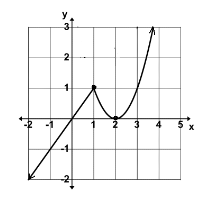
\includegraphics[width=0.3\textwidth]{2019B37.PNG}
    \end{center}

    \item % 123
    Bill Defense is fencing in a non-square rectangular area of 3,200 square feet. The cost of the fencing for two sides of the rectangle will cost $\$1.00$ per foot and the other two sides will cost $\$2.00$ per foot. What is the lowest possible cost for the fence?

    \item % 124
    Given: $f$ is a continuous function on the interval $[0,2]$ such that $\int_0^2 f(x)\dd x = 5$. Find $\int_0^1 f(2y)\dd y$.

\end{enumerate}

\section*{Solutions}
\begin{enumerate}[label=\bfseries\arabic*.]
    \item %% Problem 1
    2

    \item %% Problem 2
    C 

    \item %% Problem 3
    -6

    \item %% Problem 4
    $(0,1)$

    \item %% Problem 5
    18 

    \item %% Problem 6
    $10\frac{2}{3}$

    \item %% Problem 7
    -8.0

    \item %% Problem 8
    193

    \item %% Problem 9
    4890 

    \item %% Problem 10
    14.1

    \item %% Problem 11
    $(-4,4)$

    \item %% Problem 12
    -2.24

    \item %% Problem 13
    $\sin x$

    \item %% Problem 14
    $2x+h-8, h\neq 0$

    \item %% Problem 15
    21.0

    \item %% Problem 16
    -1.5

    \item %% Problem 17
    0.02 rad/s 

    \item %% Problem 18
    407.9 in$^3$

    \item %% Problem 19
    114

    \item %% Problem 20
    102.7

    \item %% Problem 21
    $4\sin(4x)$

    \item %% Problem 22
    $x^2$

    \item %% Problem 23
    0.0000021

    \item %% Problem 24
    1.6

    \item %% Problem 25
    $\frac{1}{2}$

    \item %% Problem 26
    6.7

    \item %% Problem 27
    36.4

    \item %% Problem 28
    Intermediate Value 

    \item %% Problem 29
    28,800 ft$^2$

    \item %% Problem 30
    3.46 in/s 

    \item %% Problem 31
    3.8

    \item %% Problem 32
    2.01

    \item %% Problem 33
    $\sin(x)$

    \item %% Problem 34
    $x^2$

    \item %% Problem 35
    242 

    \item %% Problem 36
    8.00

    \item %% Problem 37
    2.14

    \item %% Problem 38
    22.6

    \item %% Problem 39
    -4.0

    \item %% Problem 40
    85.3

    \item %% Problem 41
    6434

    \item %% Problem 42
    0.222

    \item %% Problem 43
    5.9

    \item %% Problem 44
    51,200

    \item %% Problem 45
    7 in/s 

    \item %% Problem 46
    52.7

    \item %% Problem 47
    -0.27 m/s 

    \item %% Problem 48
    -1.0 m/s$^2$

    \item %% Problem 49
    4530

    \item %% Problem 50
    642

    \item %% Problem 51
    50.6

    \item %% Problem 52
    $-\frac{2^{-x}}{\ln 2}$

    \item %% Problem 53
    5

    \item %% Problem 54
    $(1,1)$

    \item %% Problem 55
    $1\frac{1}{3}$

    \item %% Problem 56
    Mean-value Theorem 

    \item %% Problem 57
    E 

    \item %% Problem 58
    $4\frac{1}{2}$

    \item %% Problem 59
    $2\frac{3}{4}$

    \item %% Problem 60
    6

    \item %% Problem 61
    Intermediate Value Theorem 

    \item %% Problem 62
    $22a-18b$

    \item %% Problem 63
    6

    \item %% Problem 64
    1

    \item %% Problem 65
    $3x+6y$

    \item %% Problem 66
    $20\frac{5}{6}$

    \item %% Problem 67
    -22

    \item %% Problem 68
    $(2,-1)$

    \item %% Problem 69
    $-2n(n^2+5)$

    \item %% Problem 70
    -.416

    \item %% Problem 71
    Rolle's Theorem 

    \item %% Problem 72
    $1\frac{2}{3}$

    \item %% Problem 73
    $10\frac{2}{3}$

    \item %% Problem 74
    $-\frac{5}{12}$

    \item %% Problem 75
    $2x+5y=17$

    \item %% Problem 76
    -4

    \item %% Problem 77
    $y=-x$

    \item %% Problem 78
    $10\frac{2}{3}$

    \item %% Problem 79
    $x\cos x-\sin x$

    \item %% Problem 80
    17 

    \item %% Problem 81
    $-\frac{1}{16}$

    \item %% Problem 82
    $1\frac{1}{3}$

    \item %% Problem 83
    $222\frac{3}{4}$

    \item %% Problem 84
    -6 

    \item %% Problem 85
    $-\frac{1}{8}\cos(4x)$

    \item %% Problem 86
    7000 sq. ft.

    \item %% Problem 87
    $10\frac{2}{3}$

    \item %% Problem 88
    -4

    \item %% Problem 89
    $\frac{y-1}{1-x}$

    \item %% 90
    2

    \item %% 91
    1 \& 2 but not 3 

    \item %% 92
    -11

    \item % 93
    6.5

    \item % 94
    2.5

    \item % 95
    4.5 ft/sec 

    \item % 96
    2

    \item % 97
    3 only 

    \item % 98
    102'0''

    \item % 99
    4.25

    \item % 100
    -1

    \item % 101
    126 cm$^2$/min 

    \item % 102
    -2

    \item % 103
    3

    \item % 104
    1

    \item % 105
    4.5

    \item % 106
    8.9

    \item % 107
    19.0

    \item % 108
    13.6

    \item % 109
    49.3

    \item % 110
    $\sin(2)$

    \item % 111
    34.5

    \item % 112
    55.11

    \item % 113
    2385

    \item % 114
    151$\degree$

    \item % 115 
    I, III only 

    \item % 116
    2.09 cm/s 

    \item % 117
    9.63 cm 

    \item % 118
    258

    \item % 119
    $12x-23$

    \item % 120
    $2\frac{1}{4}$

    \item % 121
    $-6$

    \item % 122
    $x<1$ and $x>1$

    \item % 123
    $\$320.00$

    \item % 124
    2.5


\end{enumerate}


\end{document}